%%
%% This is file `main.tex'
%%
%% ------------------------------------------------------------------------
%% Copyright (C) 2022 Q.Tang
%% 
%% Licensed under the Apache License, Version 2.0 (the "License");
%% you may not use this file except in compliance with the License.
%% You may obtain a copy of the License at
%% 
%%     http://www.apache.org/licenses/LICENSE-2.0
%% 
%% Unless required by applicable law or agreed to in writing, software
%% distributed under the License is distributed on an "AS IS" BASIS,
%% WITHOUT WARRANTIES OR CONDITIONS OF ANY KIND, either express or implied.
%% See the License for the specific language governing permissions and
%% limitations under the License.
%% ------------------------------------------------------------------------

\documentclass{bjtu-bachelor-thesis}
%========================================================================%
% 自定义内容
%========================================================================%

\author{XX}
\studentNumber{1730xxxx}
\advisor{XXX}
\school{软件学院}
\major{软件工程}
\title{设计(论文)题目}
\englishtitle{The Design and Implementation of \\ Thesis Template Based on \LaTeX}

%========================================================================%
% 前置部分
%========================================================================%

\begin{document}
\pagenumbering{roman}
\makecover % 封面
\makeAuthorization % 版权声明

\setcounter{page}{1}
\pagestyle{bjtufancy}

\begin{chineseabstract}	

\noindent\bjtusongti{\textbf{摘要:}}[鼠标左键单击选择该段落,输入替换之。内容为小四号宋体。] 中文摘要应将论文的内容要点简短明了地表达出来,约400字左右,字体为宋体小四号。内容应包括工作目的、研究方法、成果和结论。要突出本论文的创新点,语言力求精炼。为了便于文献检索,应在本页下方另起一行注明论文的关键词(3-5个),如有可能,尽量采用《汉语主题词表》等词表提供的规范词。图X幅,表X个,参考文献X篇。\par

	\vspace{2cm}
	
	\noindent \bjtusongti {\textbf{关键词:}[请输入关键词(3-5),以分号分隔。] }
\end{chineseabstract}
 % 中文摘要
\begin{englishabstract}

	\noindent\bjtusongti{\textbf{ABSTRACT:}} 
	
	\noindent "[鼠标左键单击选择该段落,输入替换之。内容为小四号Times New Roman。]" 与中文摘要内容要相对应。 \par

	\vspace{2cm}
	
	\noindent \bjtusongti {\textbf{KEYWORDS:\;}[请输入英文关键词,与中文关键词保持一致。以分号分隔。]  } 
\end{englishabstract} % 中文摘要

% 目录
\tableofcontents
\addcontentsline{toc}{part}{目\hspace{2em}录}%
\pagestyle{bjtufancy}
%========================================================================%
% 主体部份
%========================================================================%

\newpage
\pagestyle{bjtufancymain}
\setcounter{page}{1}
\pagenumbering{arabic}

\chapter{引言}
\markboth{正文}{正文}

\setlength{\baselineskip}{20pt}

本章将主要介绍深度图像超分辨率重建的研究背景、研究现状、研究难点以及本文的研究内容与主要贡献。本章的组织结构如下:第一部分主要介绍深度图像超分辨率重建的研究背景以及该任务在实际应用中的研究意义和价值,第二部分将介绍深度图像超分辨率重建和单目深度估计的研究现状以及将两个任务统一于一个网络框架联合学习的主要难点,第三部分将介绍本文的主要研究内容和贡献,最后介绍论文的结构安排。

\section{研究背景与实际应用}

在理解场景时,人们不仅可以感知其外观(例如颜色,纹理等),还可以捕获深度信息以产生立体感。更好的场景理解可以促进自动驾驶 \cite{DBLP:conf/iros/KerlSC13},三维重建 \cite{DBLP:journals/pami/ImHCJJK19} 等依赖于高质量和高分辨率深度信息领域的研究。便携式消费级深度相机(如 Microsoft Kinect 和 Lidar)的出现和普及,为准确快速地获取场景深度提供了极大的便利。但是,由于当前深度相机成像能力的限制,深度图像的分辨率通常较低,无法与同场景的高分辨率彩色图像相匹配。面对诸多应用领域对高质量深度图像的需求 \cite{DBLP:journals/corr/abs-1907-06781, DBLP:journals/pami/GeLYT19, SilbermanHKF12},深度图像超分辨率重建技术作为解决方案获得了越来越多的关注。

深度图像超分辨率重建技术是指在不改变深度相机或深度传感器的前提下,通过算法恢复出相机或传感器截止频率以外的高频信息(图像的高频信息是指灰度变化快速的区域,例如物体边缘),同时改善成像时的模糊现象并有效抑制图像中的随机噪声,从而重建出高质量、高分辨率的深度图像。传统的基于滤波的方法 \cite{0001TT13,LuSMLD12} 和基于优化的方法 \cite{DBLP:conf/iccv/FerstlRRRB13, ParkKTBK11} 使用人工构造的滤波器或目标函数很难恢复出准确的高分辨率深度图像。近年来,随着深度学习的快速发展,许多研究已经表明了其在深度图像超分辨率重建任务上的有效性 \cite{HuiLT16, WenSLLF19}。基于卷积神经网络的深度图像超分辨率重建技术可以自动地从数据中学习更强的特征表示来重建高分辨率深度图像。

在实际应用中,高分辨率的彩色图像易于获得,且与深度图像具有很强的结构相似性,因而可以为深度图像超分辨率重建提供一些先验信息。这种利用彩色图像引导的深度图像超分辨率重建算法被称为颜色(或纹理图像)指导的深度图像超分辨率重建算法。现有的颜色指导的深度图像超分辨率重建算法通常需要一个额外的分支来从彩色图像中获取丰富的指导信息 \cite{LutioDWS19},然后利用它们来指导超分辨率重建分支对深度图像的特征提取。但是,彩色图像的结构并不总是与深度图像相一致。如 \ref{fig:1-1} 示,绿色矩形区域在彩色图像上具有复杂的纹理变化,但是由于目标内部的深度一致性,在对应的深度图像中该区域并没有表现出对应的纹理结构。因此,如果仅将从彩色图像提取的特征或边缘特征传递到超分辨率重建分支,就很容易造成诸如纹理复制和深度流失等问题。因此,探索如何有效地提取和利用高分辨率彩色图像蕴含的信息对于深度图像超分辨率重建任务非常重要。

\begin{figure}[!htbp]
\vspace{-0.8cm}  %调整图片与上文的垂直距离
	\centering
	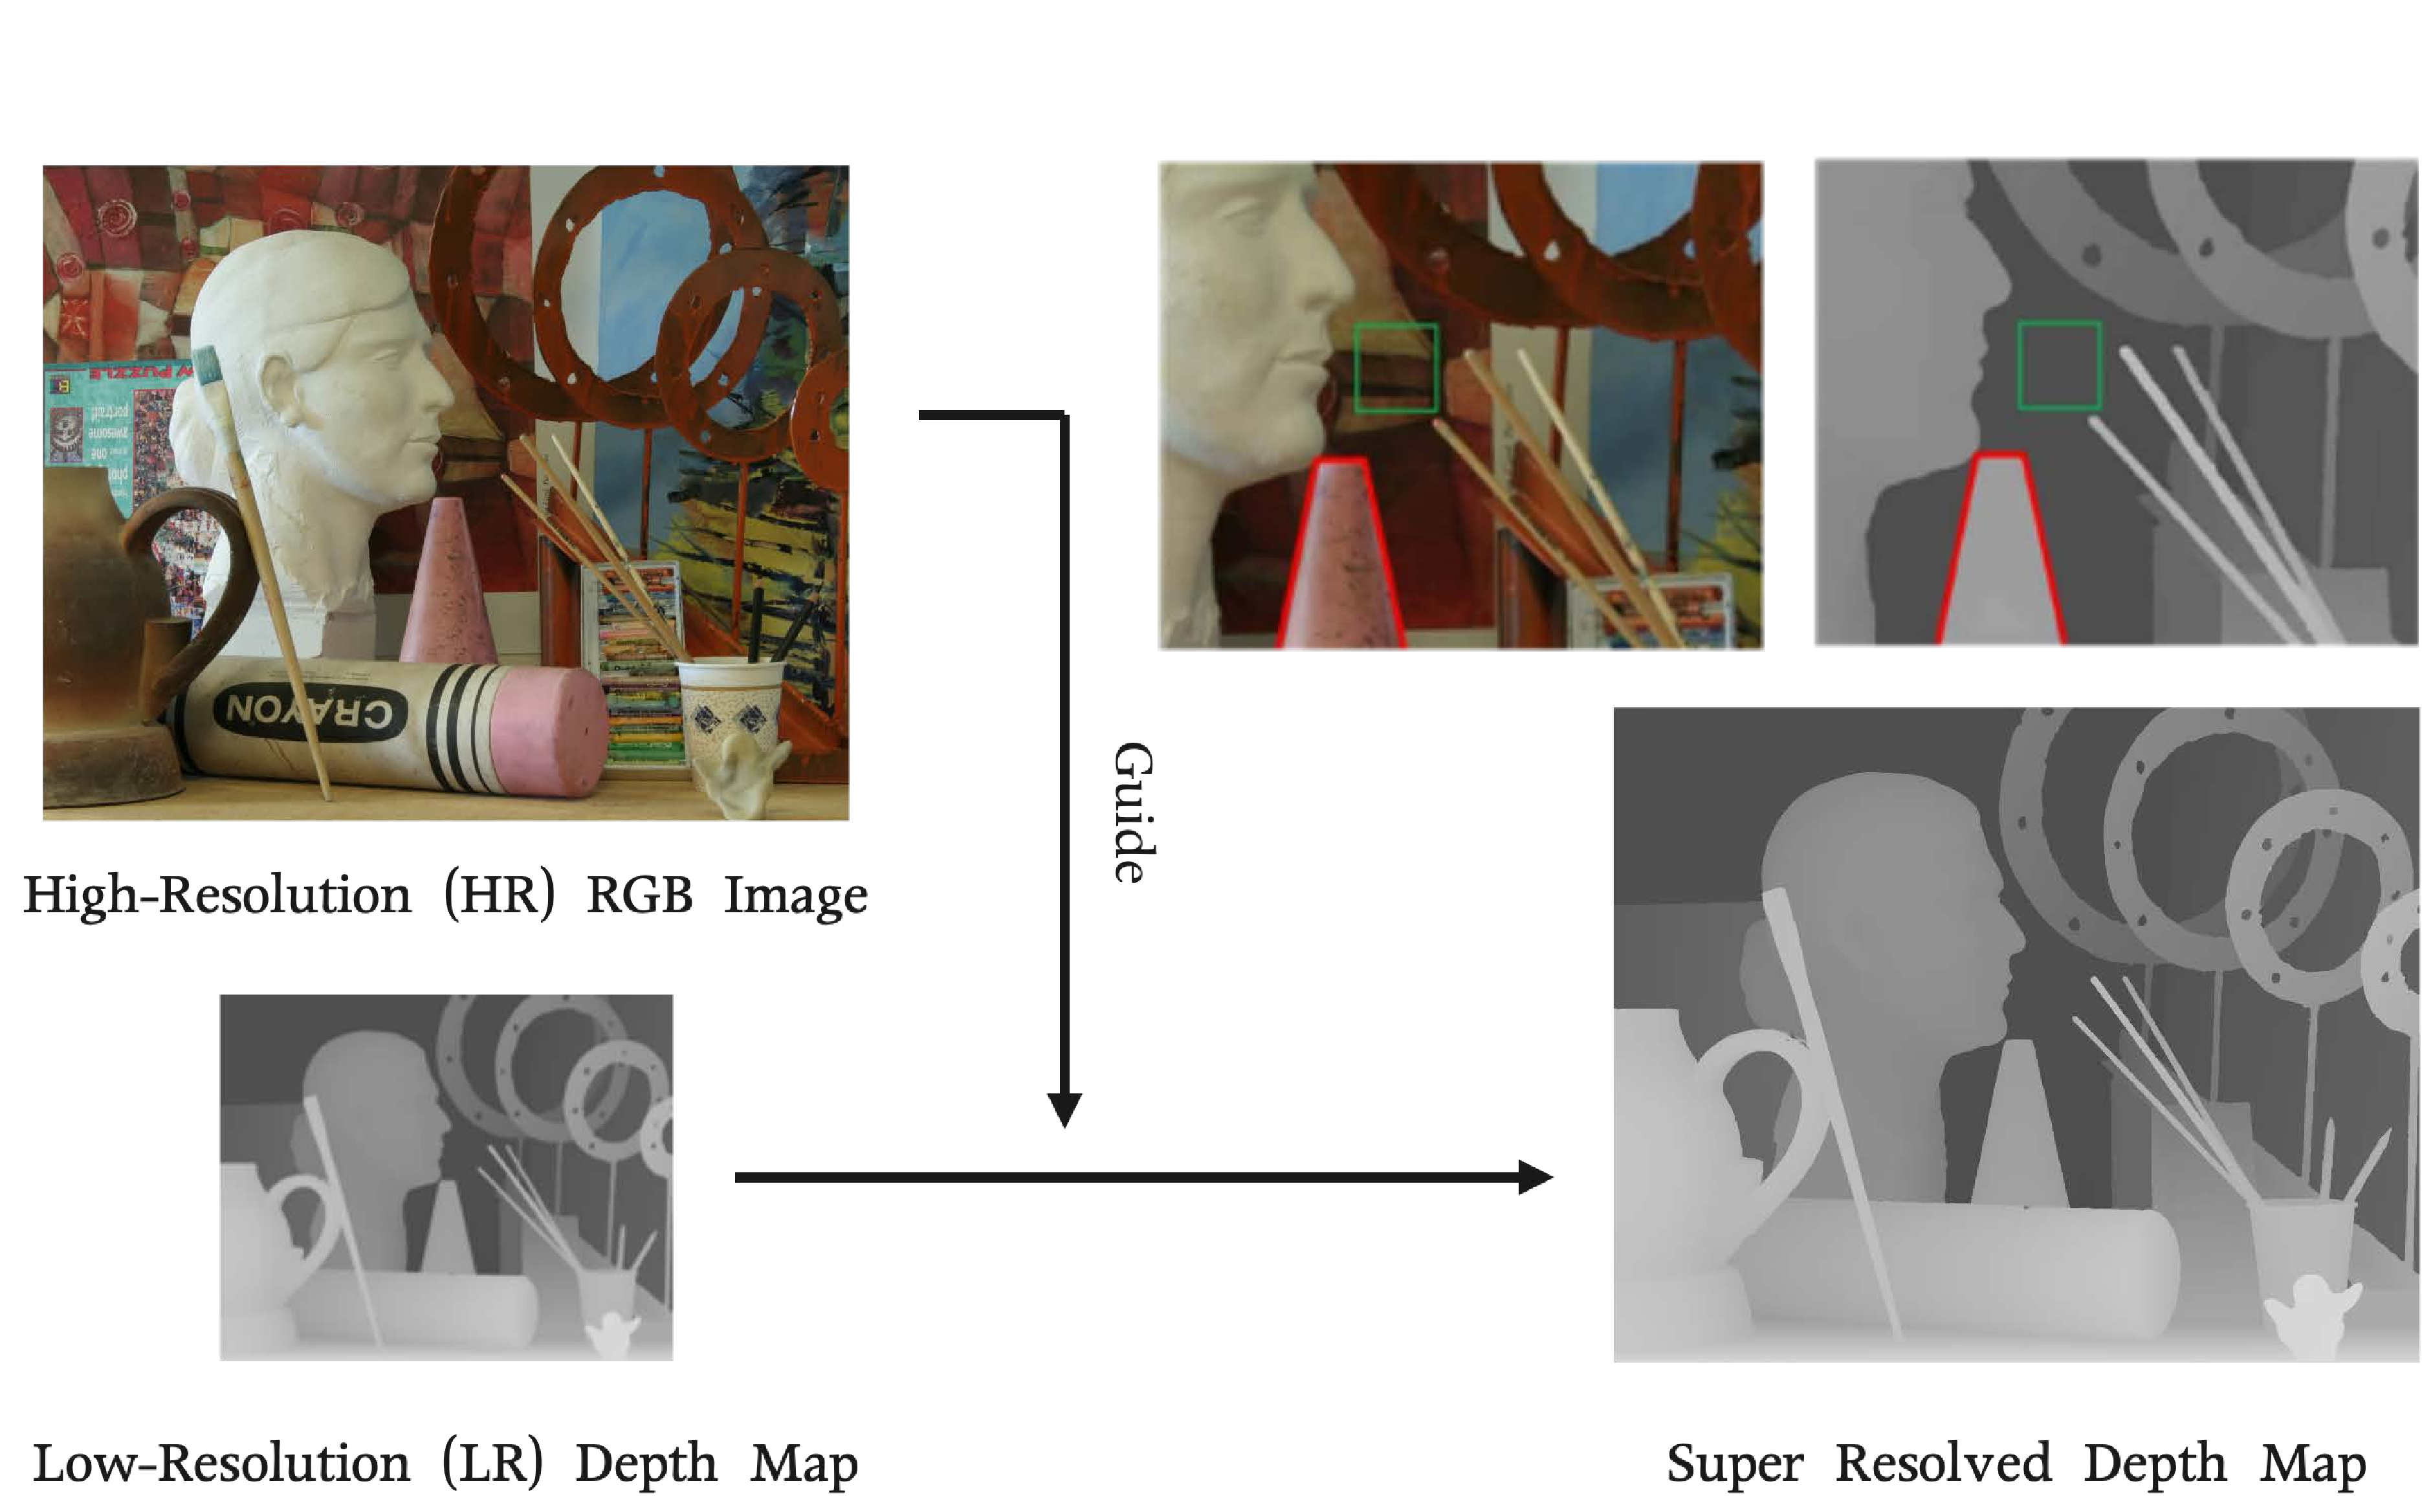
\includegraphics[scale=0.14]{figures/1}
	\caption{颜色引导的深度图像超分辨率重建示意图}
	\label{fig:1-1}
\end{figure}

为了寻找上述问题的解决方案,本文将目光聚焦在了另一个与深度图像有关的任务——单目深度估计。单目深度估计旨在将场景从光度表示映射到几何表示。具体而言,单目深度估计的输入是一幅彩色图像,而输出则是估计的深度图像。

单目深度估计与深度图像超分辨率重建两个任务是天然相关的:
\begin{enumerate}
	\item[(1)]	将两个任务嵌入联合学习的训练框架中,无需引入额外的监督标签(例如语义标签),即两个任务的训练数据集可以共享。
	\item[(2)] 由于单目深度估计可以在连续的训练和学习过程中实现从彩色图像到深度图像的跨模态信息转换,因而面向单目深度估计学习到的彩色图像特征更适合指导深度图像超分辨率重建。
\end{enumerate}

综上所述,深度图像超分辨率重建与单目深度估计的联合学习可以在不增加监督信息的情况下实现更好的颜色指导。

\section{研究现状及难点}

本部分将分别介绍深度图像超分辨率重建和单目深度估计的研究现状,并将详细分析将单目深度估计与深度图像超分辨率重建统一于联合学习框架的难点。

\subsection{深度图像超分辨率重建}

由于彩色图像和深度图像间的结构相似性,现有的许多方法都利用颜色信息指导低分辨率深度图像的重建。Zhao 等 \cite{DBLP:journals/corr/abs-1708-09105} 提出提出了彩色-深度条件生成对抗网络(Color-Depth Conditional Generative Adversarial Network, CDcGAN)来同时解决3D视频中的深度图像和彩色图像超分辨率重建问题,该网络考虑了同一场景下彩色图像和深度图像的结构相似性,采用彩色图像和深度图像的交互信息来相互促进彼此的性能。 Hui 等 \cite{HuiLT16} 设计了多尺度引导的卷积神经网络(Multi-Scale Guided convolutional network, MSG),将从彩色图像中提取的丰富层次特征用于改善深度图像超分辨率重建过程中图像的模糊现象。 Zuo 等 \cite{DBLP:journals/isci/ZuoFYSW19} 提出了彩色引导的深度图像增强残差稠密网络(Residual Dense Network for Guided Depth Enhancement, RDN-GDE),将多尺度残差与稠密连接相结合以逐步增强低分辨率的深度图像。 Ye 等 \cite{DBLP:journals/tip/YeSWYXLL20} 提出了渐进的多分支聚合网络(Progressive Multi-Branch Aggregation network, PMBA), 通过重建分支和引导分支融合的方式逐步优化反卷积得到的高分辨率深度图像。 Guo 等 \cite{DBLP:journals/tip/GuoLGCFH19} 提出了层次特征驱动的深度图像超分辨率重建残差网络 DepthSR-Net, 利用 U-Net 结构对插值后的深度图像进行编码,并在解码过程中与相应尺度的彩色特征进行融合。

\subsection{单目深度估计}

单目深度估计是一个典型的不适定逆问题,这是由于其将在信息不足以完全指定解决方案的情况下尝试恢复一些未知数。与基于左右视图的深度估计任务相比,单目深度估计具有更加广阔的实际应用前景,但目前单目深度估计的性能仍然非常有限。Eigen 等 \cite{DBLP:conf/nips/EigenPF14} 设计了一个包含对场景全局的粗估计和局部区域的精估计两个尺度的卷积神经网络,开创了深度学习在单目深度估计领域的先河。Laina等 \cite{DBLP:conf/3dim/LainaRBTN16} 使用了更深的残差网络并通过小卷积进行上采样,从而提升了单目深度估计的效率。Cao等 \cite{DBLP:journals/tcsv/CaoWS18} 将原始的连续深度离散为固定数量的深度范围,进而将单目深度估计从回归任务转换为分类任务,观察到了明显的性能提升。

\subsection{面向深度图像的多任务联合学习}

多任务学习的目的是通过相关任务联合以提升特定任务的性能,最简单的联合方法是通过损失函数将两个或多个任务组合在一起。但由于在网络设计中缺乏交互性,这通常不是最佳的策略。目前,许多与深度图像处理有关的任务都采用了多任务学习策略。Zhang 等 \cite{DBLP:conf/eccv/ZhangCXJLY18} 提出的联合任务递归学习(Joint Task-Recursive Learning, TRL)框架将问题序列化为任务交替的时间序列来递归地优化语义分割和单目深度估计任务的结果。这类方法仅仅通过网络和损失约束的设计来驱动两个任务的联合学习,而没有明确地探究任务之间存在的约束。He等 \cite{DBLP:journals/corr/abs-2101-07422} 基于两个任务的几何约束提出联合语义分割的单目深度估计网络(Semantic Object Segmentation and Depth Estimation Network, SOSD-Net)这一工作明确探究了多任务学习中任务之间的关联性,但单目深度估计和语义分割的相关性仍然较弱。此外,相对于单目深度估计而言,这些方法在训练时需要引入额外的标签(如语义标签)。Sun 等 \cite{Sun2021cvpr} 提出了一种通过单目深度估计在训练过程中帮助深度图像超分辨率重建更好地理解场景结构的知识蒸馏方法,从而证明了单目深度估计在改善深度图像超分辨率重建性能方面的有效性。但其通过比较训练过程中两个任务的平均像素误差来确定两个任务交互方向的方法,并没有明确地探究深度图像超分辨率重建与单目深度估计的相关性。

综上,联合单目深度估计的深度图像超分辨率重建的研究难点在于探究两个任务的关联性并设计合理的交互方式,尤其是探究如何将深度估计学习到的“知识”通过多任务学习的模式帮助低分辨率的深度图像进行超分辨率重建,从而达到更好的重建效果。


\section{本文主要工作}

受上述分析的驱动,本文提出了深度图像超分辨率重建和单目深度估计的联合学习网络(BridgeNet),关注于通过有效地桥接两个任务以实现更好的深度图像超分辨率重建。本文基于编码器-解码器(Encoder-Decoder)结构分别为单目深度估计和深度图像超分辨率重建任务设计了两个子网络,即深度图像超分辨率重建子网络(DSRNet)和单目深度估计子网络(MDENet),它们以多任务学习的模式协同工作。此外,本文还分别在编码器和解码器中设计了两个不同的桥接器(Bridge)以实现两个子网络的差异化引导。具体而言,单目深度估计子网络的编码器从彩色图像中学习面向深度图像的多级特征,这样的彩色特征更适用于指导深度图像的超分辨率重建。因此,本文提出了一个高频注意力桥(HABdg),将单目深度估计学习到的高频信息用于指导深度图像超分辨率重建。 单目深度估计子网络和深度图像超分辨率重建子网络的特征解码器用于进一步提取面向任务的特征,以进行深度估计和深度图像超分辨率重建。由于单目深度估计存在的尺度模糊性,单目深度估计相较于深度图像的超分辨率重建更难达到良好的性能。因此,遵循简单任务指导困难任务的原则,本文提出了内容引导桥(CGBdg),旨在使深度图像超分辨率重建子网络在深度特征空间为单目深度估计子网络提供内容引导。除了在模型设计层面上关联这两个任务外,本文还在损失函数方面对其进行约束,以期两个子网络可以相互促进。

综上所述,本文主要贡献如下:
\begin{enumerate}[leftmargin=55bp]
\item[(1)]	本文在联合学习网络中将深度图像超分辨率重建任务和单目深度估计任务相关联,以提升深度图像超分辨率重建的性能。本文提出的联合学习网络包括深度图像超分辨率重建子网络(DSRNet)和单目深度估计子网络(MDENet),以及两个用于联合学习的桥接器,即高频注意力桥(HABdg)和内容引导桥(CGBdg)。本文的整个网络结构具有高度的可移植性,可以为关联深度图像超分辨率重建和单目深度估计任务提供范例。此外,与其他多任务学习不同,本文用于联合学习的两个任务不需要引入其他的监督信息。  
\item[(2)]	 特征编码阶段中的高频注意力桥(HABdg)将从单目深度估计子网络学习到的彩色高频信息传输到深度图像超分辨率重建子网络,从而可以提供更接近深度模态的颜色指导信息。遵循简单任务指导困难任务的原则,本文在特征解码阶段切换了两个任务的指导角色,并提出了内容引导桥(CGBdg),从而可以让深度图像超分辨率重建子网络在深度特征空间为单目深度估计子网络提供内容引导。
\item[(3)]	在不引入其他监督信息的情况下,本文的方法在多个公开基准数据集上均达到了具有竞争力的性能。 
\end{enumerate}


\section{结构安排}

本文一共分为五章,每一章节的内容安排如下:

第一章为引言,以深度图像超分辨率重建的研究背景和现实意义、颜色引导的深度图像超分辨率重建存在的问题、单目深度估计与深度图像超分辨率重建颜色分支的相似性为脉络层层递进,进而引出本文在多任务学习模式下将深度估计和深度图像超分辨率重建相关联的研究内容,接着分别介绍了两个任务的研究现状以及将他们统一于一个网络框架联合学习的关键难点,最后对论文的结构组织进行介绍。

第二章为相关技术和方法介绍,主要介绍了与本文研究相关的技术和方法,即联合单目深度估计的深度图像超分辨率重建网络的基石。

第三章为算法实现,详细地介绍了单目深度估计和深度图像超分辨率重建联合学习网络的架构设计,包括深度图像超分辨率重建子网络,单目深度估计子网络以及高频注意力桥和内容引导桥。

第四章为实验测试与分析,介绍了本文了采用的公开基准数据集和评估指标,然后对比分析了本文设计的网络在所选公开基准数据集上进行训练和测试的性能表现,以及与其他最新的深度图像超分辨率重建网络性能的对比。此外,通过消融实验验证了不同设计对网络性能的影响。

第五章为结论,对本文的工作进行总结,囊括了本文的主要贡献,并概述了未来工作的研究方向。


\section{本章小结}

本章层层递进地介绍了深度图像超分辨率重建的研究背景和意义,然后从颜色引导的深度图像超分辨率重建存在的问题出发,阐明了联合单目深度估计与深度图像超分辨率重建联合学习算法的研究动机,进而分别介绍了两个任务的研究现状以及探究两个任务的关联性在是设计两个任务联合学习网络的重点和难点,然后对本文的主要贡献进行了详细介绍。

\chapter{【1级标题,三号黑体字】}
 
 [鼠标左键单击选择该段落,输入替换之。内容为小四号宋或楷体字。] 学位论文为了需要反映出作者确已掌握了坚实的基础理论和系统的专门知识,具有开阔的科学视野,对研究方案作了充分论证,因此,有关历史回顾和前人工作的综合评述,以及理论分析等,可以单独成章,用足够的文字叙述。正文是学位论文的核心部分,占主要篇幅,可以包括:调查对象、实验和观测方法、仪器设备、材料原料、实验和观测结果、计算方法和编程原理、数据资料、经过加工整理的图表、形成的论点和导出的结论等。\par
由于研究工作涉及的学科、选题、研究方法、工作进程、结果表达方式等有很大的差异,对正文内容不能作统一的规定。但是,必须实事求是,客观真切,准确完备,合乎逻辑,层次分明,简练可读。\par
\textcolor{red}{\textbf{图:}}\par
图包括曲线图、构造图、示意图、框图、流程图、记录图、地图、照片等。\par
图应具有“自明性”。\par
图应有编号。图的编号由“图”和从“1”开始的阿拉伯数字组成,图较多时,可分章编号。\par
图宜有图题,图题即图的名称,置于图的编号之后。图的编号和图题应置于图下方。\par
照片图要求主题和主要显示部分的轮廓鲜明,便于制版。如用放大缩小的复制品,必须清晰,反差适中。照片上应有表示目的物尺寸的标度。\par
图片示例1:
\begin{figure}[!htbp]
    \centering
    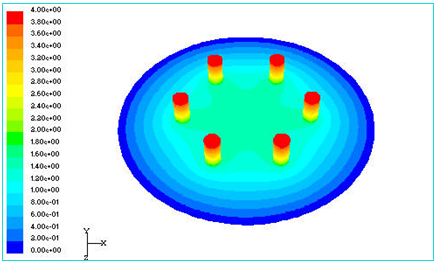
\includegraphics[width=0.5\textwidth]{figures/pic2-1.png}
    \caption{太合金多炭钢铁产品柱扭曲局部受力分析示意图}
    \label{fig:2-1}
\end{figure}

\textcolor{red}{\textbf{表:}}\par
表应具有“自明性”。\par
表应有编号。表的编号由“表”和从“1”开始的阿拉伯数字组成,表较多时,可分章编号。表较多时,可分章编号。\par
表宜有表题,表题即表的名称,置于表的编号之后。表的编号和表题应置于表上方。\par
表的编排,一般是内容和测试项目由左至右横读,数据依序竖读。\par
表的编排建议采用国际通行的三线表。\par
如某个表需要转页接排,在随后的各页上应重复表的编号。编号后跟表题(可省略)和“(续)”,置于表上方。\par
续表均应重复表头。\par
表格示例1:

\begin{table}[htbp]

    \centering
    \caption{国际单位制的基本单位}
    \label{tbl:2-1}
    \begin{tabularx}{0.8\textwidth}{*{3}{>{\centering\arraybackslash}X}}
        \toprule
        量的名称   & 单位名称     & 单位符号 \\ \midrule
        长度       & 米           & m        \\
        质量       & 千克(公斤)   & kg       \\
        时间       & 秒           & s        \\
        电流       & 安{[}培{]}   & A        \\
        热力学温度 & 开{[}尔文{]} & K        \\
        物质的量   & 摩{[}尔{]}   & mol      \\
        发光强度   & 坎{[}德拉{]} & cd       \\ \bottomrule
    \end{tabularx}
\end{table}

\textcolor{red}{\textbf{公式:}}\par
论文中的公式应另行起,并缩格书写,与周围文字留足够的空间区分开。\par
如有两个以上的公式,应用从“1”开始的阿拉伯数字进行编号,并将编号置于括号内。公式的编号右端对齐,公式与编号之间可用“…”连接。公式较多时,可分章编号。\par
公式示例1:
\begin{equation}
    \label{eqn:2}
    \phi=\frac{D_{p}^{2}}{150} \frac{\psi^{3}}{(1-\psi)^{2}}
\end{equation}
\begin{equation}
    \label{eqn:3}
    C_{2} =\frac{3.5}{D_{p}} \frac{(1-\psi)}{\psi^{3}}
\end{equation}

\noindent 式中  $\quad D_{p}$ —— 多孔质材料的平均粒子直径($m$);\par
$\psi$ —— 孔隙度(孔隙体积占总体积的百分比); \par
$\phi$ —— 特征渗透性或固有渗透性,与材料的结构性质有关($m^2$)。\par
较长的公式需要转行时,应尽可能在“=”处回行,或者在“+”、“-”“×”、“/”等记号处回行。\par
公式中分数线的横线,其长度应等于或略大于分子和分母中较长的一方。\par
如正文中书写分数,应尽量将其高度降低为一行。如将分数线书写为“/”,将根号改为负指数。\par
\newpage
公式示例2:\par
\begin{spacing}{2}
    \begin{math}
        \zihao{5} \quad\text{将}\;\dfrac{1}{\sqrt{2}}\;\text{写成}\; 1/\sqrt{2} \;\text{或}\; 2^{-1/2}。
    \end{math}
\end{spacing}

\textcolor{red}{\textbf{引文标注}}\par
论文中引用的文献的标注方法遵照GB/T 7714-2005,可采用顺序编码制,也可采用著者-出版年制,但全文必须统一。\par
\textcolor{red}{\textbf{注释}}\par
当论文中的字、词或短语,需要进一步加以说明,而又没有具体的文献来源时,用注释。注释一般在社会科学中用得较多。\par
应控制论文中的注释数量,不宜过多。\par
由于论文篇幅较长,建议采用文中编号加“脚注”的方式。最好不用采用文中编号加“尾注”。\par

\section{【2级标题,小三号黑体字】 }
 [鼠标左键单击选择该段落,输入替换之。内容为小四号宋或楷体字。]
\subsection{【3级标题,四号黑体字】 }
[鼠标左键单击选择该段落,输入替换之。内容为小四号宋或楷体字。]
\chapter{【1级标题,三号黑体字】}
\section{【2级标题,小三号黑体字】 }
 [鼠标左键单击选择该段落,输入替换之。内容为小四号宋或楷体字。]
\subsection{【3级标题,四号黑体字】 }
[鼠标左键单击选择该段落,输入替换之。内容为小四号宋或楷体字。]
\chapter{【1级标题,三号黑体字】}
\section{【2级标题,小三号黑体字】 }
 [鼠标左键单击选择该段落,输入替换之。内容为小四号宋或楷体字。]
\subsection{【3级标题,四号黑体字】 }
[鼠标左键单击选择该段落,输入替换之。内容为小四号宋或楷体字。]
\chapter{结论}
\markboth{正文}{正文}

本文探索了一种联合学习框架,该框架结合了深度图像超分辨率重建和单目深度估计两个任务,可以在不添加任何其他监督信息的情况下提升深度图像超分辨率重建的性能。

高分辨率彩色图像由于其具有与深度图像的结构相似性且容易获得,被广泛用于为深度图像超分辨率重建提供先验信息。但现有颜色指导的深度图像超分辨率重建算法通过额外分支提取到的指导信息,并没有很好地面向深度模态,因此可能在两种模态结构不一致的区域造成纹理复制等问题。而单目深度估计旨在将场景从光度表示映射到几何表示,换言之,在连续的训练和学习过程中,单目深度估计实现了从彩色图像到深度图像的跨模态信息转换。因而面向单目深度估计学习到的彩色图像特征更适合指导深度图像超分辨率重建。

本文的核心思想是如何设计两个子网络(即深度图像超分辨率重建子网络和单目深度估计子网络)之间的交互,由此本文提出了两个桥接器。特征编码阶段中的高频注意力桥将从单目深度估计子网络学习到的彩色高频信息传输到深度图像超分辨率重建子网络,从而可以提供更接近深度模态的颜色指导信息。遵循简单任务指导困难任务的原则,在特征解码阶段交换了两个任务的指导角色,深度图像超分辨率重建子网络通过内容引导桥为单目深度估计子网络在深度特征空间提供内容引导。全面的实验表明,本文提出的方法达到了具有竞争力的性能,尤其是在上采样因子较大的情况下。

此外,本文提出的网络结构具有高度的可移植性,可以为关联深度图像超分辨率重建任务和单目深度估计任务提供范例。在未来的工作中,可以通过替换不同的单目深度估计子网络和深度图像超分辨率重建子网络以更进一步验证本文提出的交互模式的普适性,并在提升深度图像超分率重建性能的同时加快网络的推理速度。


%========================================================================%
% 参考文献
%========================================================================%
\newpage
\pagestyle{bjtufancy}

\nocite{*} % 显示.bib文件中的所有参考文献,无论正文是否引用

\printbibliography[heading=bjtuheading]
\addcontentsline{toc}{part}{参考文献}
\cleardoublepage
%========================================================================%
% 致谢
%========================================================================%
%\thankspage
\begin{thanks}
故事讲了很长,感谢你一直读到这里。但故事还没有结束,写下去才知道梦有多长。

桃李不言,下自成蹊。感谢指导教师冯凤娟老师在我完成毕业论文过程中给予的悉 心指导和细致审阅,让我能把这份工作更好地呈现在论文中。从第一次在老师的课堂上 学习到完成毕业设计的选题和论文的撰写,我不仅从中获得了很多专业技能的提升,冯老师为人的热情和执教的认真也深深影响了我。谨在此以平铺直叙的话语感谢老师一直 以来的教导和帮助,祝愿老师身体健康,工作顺利。

落实思树,饮流怀源。感谢北京交通大学数字媒体信息处理研究中心赵耀老师和丛 润民老师提供的研究课题和平台,以及对我研究思路和论文写作的指导。两位老师对科 研的热忱更加激发了我对科研的神往和为之努力的斗志。在今后以梦为马的求学路上, 我必将紧随两位老师的步伐,把热爱科研的种子埋在心中。同时,也要感谢实验室帮助 我顺利完成研究课题的各位同学。

焉得谖草,言树之背。感谢家人一直以来的支持和陪伴,尤其是父母的教育理念培 育了我良好的价值观、人生观和世界观。在停课不停学的日子里,我有机会再次和父母 放飞了高三曾被放飞的风筝。跨越三年,它承载了我的梦想,也见证了我们一家的幸福 时光。父母教会的我不仅是要好好学习,更要热爱自己的生活和这个世界。祝愿我的家 人平安喜乐,幸福安康。

学贵得师,亦贵得友。感谢在红果园里每个陪我走过一段路的良师益友,在和同学 们相处的难忘岁月里,他们的优良品质影响我颇深。特别感谢在毕设期间陪在身边的三 两挚友,我们相聚一起为梦想而努力的欢乐时光必将在未来熠熠闪耀。同时,也要感谢 和我一起完成大学生创新训练计划项目的两位朋友,他们是我起航科研星空和叩开计算 机视觉大门的“梦想合伙人”。

阳和启蜇,天雨流芳。感谢一路走到现在的自己,或许神明不佑,星辰晦暗,但少 年在,光和救赎就在。别想太多,好好生活,日子过着过着就会有答案,努力走着就会 有温柔的着落。愿历经千帆,仍记得转身微笑鞠躬,向青春致敬。

喜欢高德地图的一句话:虽然前方拥堵,但您仍在最优路线上。虽然前路艰难,但 我相信最好的就快要发生。我期待着明天,前程似锦。
\end{thanks}
%========================================================================%
% 附录
%========================================================================%
\begin{appendix}

\vspace{5bp}
\noindent{\zihao{3} \heiti 附录A 外文文献及翻译}

\vspace{25bp}
\noindent{\zihao{3} \heiti 外文文献}

\vspace{25bp}
\centering{\zihao{-3}Learning Scene Structure Guidance via Cross-Task Knowledge Transfer for Single Depth Super-Resolution}

\vspace{20bp}
\centering{\zihao{5}Baoli Sun$^1$, Xinchen Ye$^{1,2*}$, Baopu Li$^3$, Haojie Li$^{1,2}$, Zhihui Wang$^{1,2}$, Rui Xu$^{1,2}$

$^1$International School of Information Science \& Engineering, Dalian University of Technology, China\newline
$^2$Key Laboratory for Ubiquitous Network and Service Software of Liaoning Province, China\newline
$^3$Baidu Research, USA
}

\vspace{25bp}
\noindent \justifying{\bfseries{Abstract.}} Existing color-guided depth super-resolution (DSR) approaches require paired RGB-D data as training samples where the RGB image is used as structural guidance to recover the degraded depth map due to their geometrical similarity. However, the paired data may be limited or expensive to be collected in actual testing environment. Therefore, we explore for the first time to learn the cross-modality knowledge at training stage, where both RGB and depth modalities are available, but test on the target dataset, where only single depth modality exists. Our key idea is to distill the knowledge of scene structural guidance from RGB modality to the single DSR task without changing its network architecture. Specifically, we construct an auxiliary depth estimation (DE) task that takes an RGB image as input to estimate a depth map, and train both DSR task and DE task collaboratively to boost the performance of DSR. Upon this, a cross-task interaction module is proposed to realize bilateral cross-task knowledge transfer. First, we design a cross-task distillation scheme that encourages DSR and DE networks to learn from each other in a teacher-student role-exchanging fashion. Then, we advance a structure prediction (SP) task that provides extra structure regularization to help both DSR and DE networks learn more informative structure representations for depth recovery. Extensive experiments demonstrate that our scheme achieves superior performance in comparison with other DSR methods. Our code available at: https://github.com/Sunbaoli/dsr-distillation.






\end{appendix}

\end{document}
